% This file was created by tikzplotlib v0.9.2.
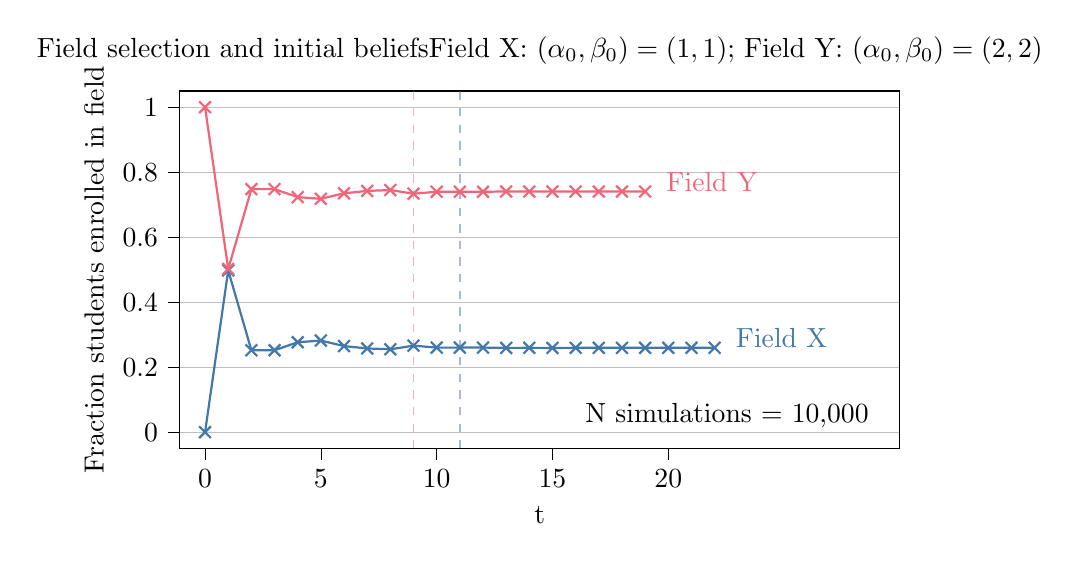
\begin{tikzpicture}

\definecolor{color0}{rgb}{0.266666666666667,0.466666666666667,0.666666666666667}
\definecolor{color1}{rgb}{0.933333333333333,0.4,0.466666666666667}

\begin{axis}[
height=6.121302808757603cm,
tick align=outside,
tick pos=left,
title={Field selection and initial beliefs \\ Field X: \(\displaystyle (\alpha_{0}, \beta_{0}) = (1, 1)\); Field Y: \(\displaystyle (\alpha_{0}, \beta_{0}) = (2, 2)\)},
unbounded coords=jump,
width=10.729849cm,
x grid style={white!69.0196078431373!black},
xlabel={t},
xmin=-1.1, xmax=30,
xtick style={color=black},
xtick={0,5,10,15,20},
xticklabels={\(\displaystyle 0\),\(\displaystyle 5\),\(\displaystyle 10\),\(\displaystyle 15\),\(\displaystyle 20\)},
ylabel={Fraction students enrolled in field},
ymajorgrids,
ymin=-0.05, ymax=1.05,
ytick style={color=black},
ytick={0,0.2,0.4,0.6,0.8,1},
yticklabels={\(\displaystyle 0\),\(\displaystyle 0.2\),\(\displaystyle 0.4\),\(\displaystyle 0.6\),\(\displaystyle 0.8\),\(\displaystyle 1\)}
]
\addplot [thick, color0, mark=x, mark size=3, mark options={solid}]
table {%
0 0
1 0.4978
2 0.2521
3 0.2521
4 0.2767
5 0.2819
6 0.2649
7 0.2576
8 0.255
9 0.2662
10 0.2602
11 0.2602
12 0.2603
13 0.2593
14 0.2595
15 0.2592
16 0.2595
17 0.2595
18 0.2595
19 0.2595
20 0.2595
21 0.2595
22 0.2596
};
\addplot [thick, color1, mark=x, mark size=3, mark options={solid}]
table {%
0 1
1 0.5022
2 0.7479
3 0.7479
4 0.7233
5 0.7181
6 0.7351
7 0.7424
8 0.745
9 0.7338
10 0.7398
11 0.7398
12 0.7397
13 0.7407
14 0.7405
15 0.7408
16 0.7405
17 0.7405
18 0.7405
19 0.7405
20 nan
21 nan
22 nan
};
\addplot [semithick, color0, opacity=0.5, dashed]
table {%
11 -0.05
11 1.05
};
\addplot [semithick, color1, opacity=0.5, dashed]
table {%
9 -0.05
9 1.05
};
\draw (axis cs:22.5,0.2596) node[
  anchor=base west,
  text=color0,
  rotate=0.0
]{Field X};
\draw (axis cs:19.5,0.7405) node[
  anchor=base west,
  text=color1,
  rotate=0.0
]{Field Y};
\draw (axis cs:16,0.03) node[
  anchor=base west,
  text=black,
  rotate=0.0
]{N simulations = 10,000};
\end{axis}

\end{tikzpicture}
